\chapter{Topology of the model and vicinity information}
\label{chapter:vicinity}

In the basic model of minority games all agents act independently without the ability to communicate with each other.
Only means of passing information between them is by using the history of the model that encapsulates all the decisions made by agents in a string of bits.
This simple model allows us to study certain characteristics of competitive systems with limited resources, however it is not a realistic assumption to think of agents as isolated elements that don't communicate with their neighbours.

Once the information of the neighbouring agents is added to the model, two important factors start to influence the dynamics of the system, (i) the dimension of the vicinity, ie. the quantity of neighbouring agents and (ii) the topology of the network generated.

In this chapter we introduce various structures used to model vicinity and how they influence the information flow in the system.
Before diving into vicinity structures, the modifications of the basic model of minority games to include local information is defined in \ref{sec:model modifications}.
First sections, \ref{sec:fixed communities} and \ref{sec:sliding communities}, refer to rather simple structures that are computationally easy to implement and maintain, however they do not express much similarity with real world applications. 
Another similar structure is explained in \ref{sec:von neumann} based on von Neumann distance. 
In the later sections, \ref{sec:scale free}, \ref{sec:small world} and \ref{sec:hierarchical vicinity}, more complex structures are introduced based on graph theory that simulate real world examples more closely. 

\section{Model modifications to include local information}
\label{sec:model modifications}

Once decided to make available new information to agents, we need to decide what that information should be and how will it be used by agents.

Information that we decided to include is the results of reduced minority games consisting of agents in the community.
In addition to global minority game, additional $C$ minority games are added, where $C$ is the number of communities that we want to include.
Each minority game follows the same definitions from Chapter \ref{chapter:minority} and the information generated is available to the agents that define the community. 
Another convention used here is that each minority game contains the same quantity of information available as the global minority game, meaning that if the length of the string of bits representing history is equal to $M$, then also the local history remembered should be $M$ bits long.

To incorporate this change in our basic model the simplest way is to create new kind of agents, called \textit{community agents}, that have the same behaviour, but their brain size is doubled.
By doubling the brain size, we do not have to change the implementation of strategies, only the history that is passed as argument to each strategy. 
For example, a strategy of a new community agent with brain size $2$ is generated is the same fashion as a strategy of a basic agent with brain size $4$ is generated.
A strategy for community agent with brain size $2$ is visible in figure \ref{table:communityStrategy} where first 2 bits, denominated local, are generated by the community minority game of the agent, and second 2 bits, denominated global, are generated by minority game consisting of all the agents.

\begin{table}
\centering
\begin{tabular}{|l|l||l|l| |c|}
\hline
\multicolumn{2}{|c||}{local}&
\multicolumn{2}{|c||}{global}&
\multicolumn{1}{|c|}{prediction} \\
\hline
\hline
0 & 0 & 0 & 1 & 1   \\ \hline
0 & 0 & 1 & 1 & 0   \\ \hline
0 & 1 & 0 & 0 & 0   \\ \hline
0 & 1 & 1 & 1 & 1   \\ \hline
1 & 0 & 0 & 0 & 0   \\ \hline
1 & 0 & 1 & 1 & 0   \\ \hline
1 & 1 & 0 & 0 & 1   \\ \hline
1 & 1 & 1 & 0 & 0   \\ \hline
\end{tabular}
\caption{Example strategy of a community agent with brain size 2}
\label{table:communityStrategy}
\end{table}

One particular case that should be noted is that by dividing the agents in communities, depending on the procedure used, a minority game where the number of agents is pair can occur.
In this case additional guard should be put in the simulation to generate a random winning side when the attendance is equal to $\frac{N}{2}$.
Of course certain procedures are implemented to reduce the number of community minority games with pairwise number of agents to minimum in order to reduce the influence on the whole model. 
Using simple structures this condition does not usually present itself, however when more complex structures are implemented it occurs with higher frequency.
Ad hoc procedures have been implemented in this thesis to reduce the number of pairwise minority games when using scale free and small world structures.

\section{Fixed one-dimensional communities}
\label{sec:fixed communities}

The simplest approach to include local information inside the model is to divide agents in certain number of communities.
By using a one-dimensional list to represent agents we can divide the array in equal parts to model communities.
Let's assume $N$ the number of agents, and $C$ number of communities, the communities are defined as
\begin{displaymath}
C_i = \bigcup agent_j \qquad|\qquad j\in [i, i+\frac{N}{C})
\end{displaymath}
An example division can be seen in figure \ref{fig:fixed vicinity} where a set of $15$ agents is divided in $5$ communities.
When the rest of $\frac{N}{C}$ is different from zero, last $N$ mod $C$ agents are assigned to their own community.

\begin{figure}
\begin{center}
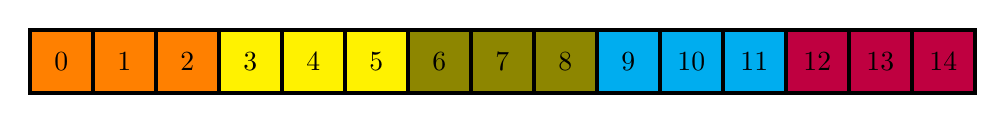
\begin{tikzpicture}[scale=0.8]
\draw [fill=orange,ultra thick] (0,0) rectangle (1,1);
\draw [fill=orange,ultra thick] (1,0) rectangle (2,1);
\draw [fill=orange,ultra thick] (2,0) rectangle (3,1);
\draw [fill=yellow,ultra thick] (3,0) rectangle (4,1);
\draw [fill=yellow,ultra thick] (4,0) rectangle (5,1);
\draw [fill=yellow,ultra thick] (5,0) rectangle (6,1);
\draw [fill=olive,ultra thick] (6,0) rectangle (7,1);
\draw [fill=olive,ultra thick] (7,0) rectangle (8,1);
\draw [fill=olive,ultra thick] (8,0) rectangle (9,1);
\draw [fill=cyan,ultra thick] (9,0) rectangle (10,1);
\draw [fill=cyan,ultra thick] (10,0) rectangle (11,1);
\draw [fill=cyan,ultra thick] (11,0) rectangle (12,1);
\draw [fill=purple,ultra thick] (12,0) rectangle (13,1);
\draw [fill=purple,ultra thick] (13,0) rectangle (14,1);
\draw [fill=purple,ultra thick] (14,0) rectangle (15,1);

\node at (0.5,.5) {0};
\node at (1.5,.5) {1};
\node at (2.5,.5) {2};
\node at (3.5,.5) {3};
\node at (4.5,.5) {4};
\node at (5.5,.5) {5};
\node at (6.5,.5) {6};
\node at (7.5,.5) {7};
\node at (8.5,.5) {8};
\node at (9.5,.5) {9};
\node at (10.5,.5) {10};
\node at (11.5,.5) {11};
\node at (12.5,.5) {12};
\node at (13.5,.5) {13};
\node at (14.5,.5) {14};
\end{tikzpicture}
\caption{Example of 15 agents divided in 5 communities, consisting of 3 agents each}
\label{fig:fixed vicinity}
\end{center}
\end{figure}

This structure creates isolated communities and only way for information to flow between communities is through the global state.
Same local information is available for each agent of the community and it is expected that this information will be used efficiently as they are all involved in the same minority game at a local level. 
However this sort of connectivity between agents does not represent real world examples as in most scenarios communities are not isolated from each other.

\begin{figure}[h]
        \centering
        \begin{subfigure}[b]{0.5\textwidth}
        	\centering
                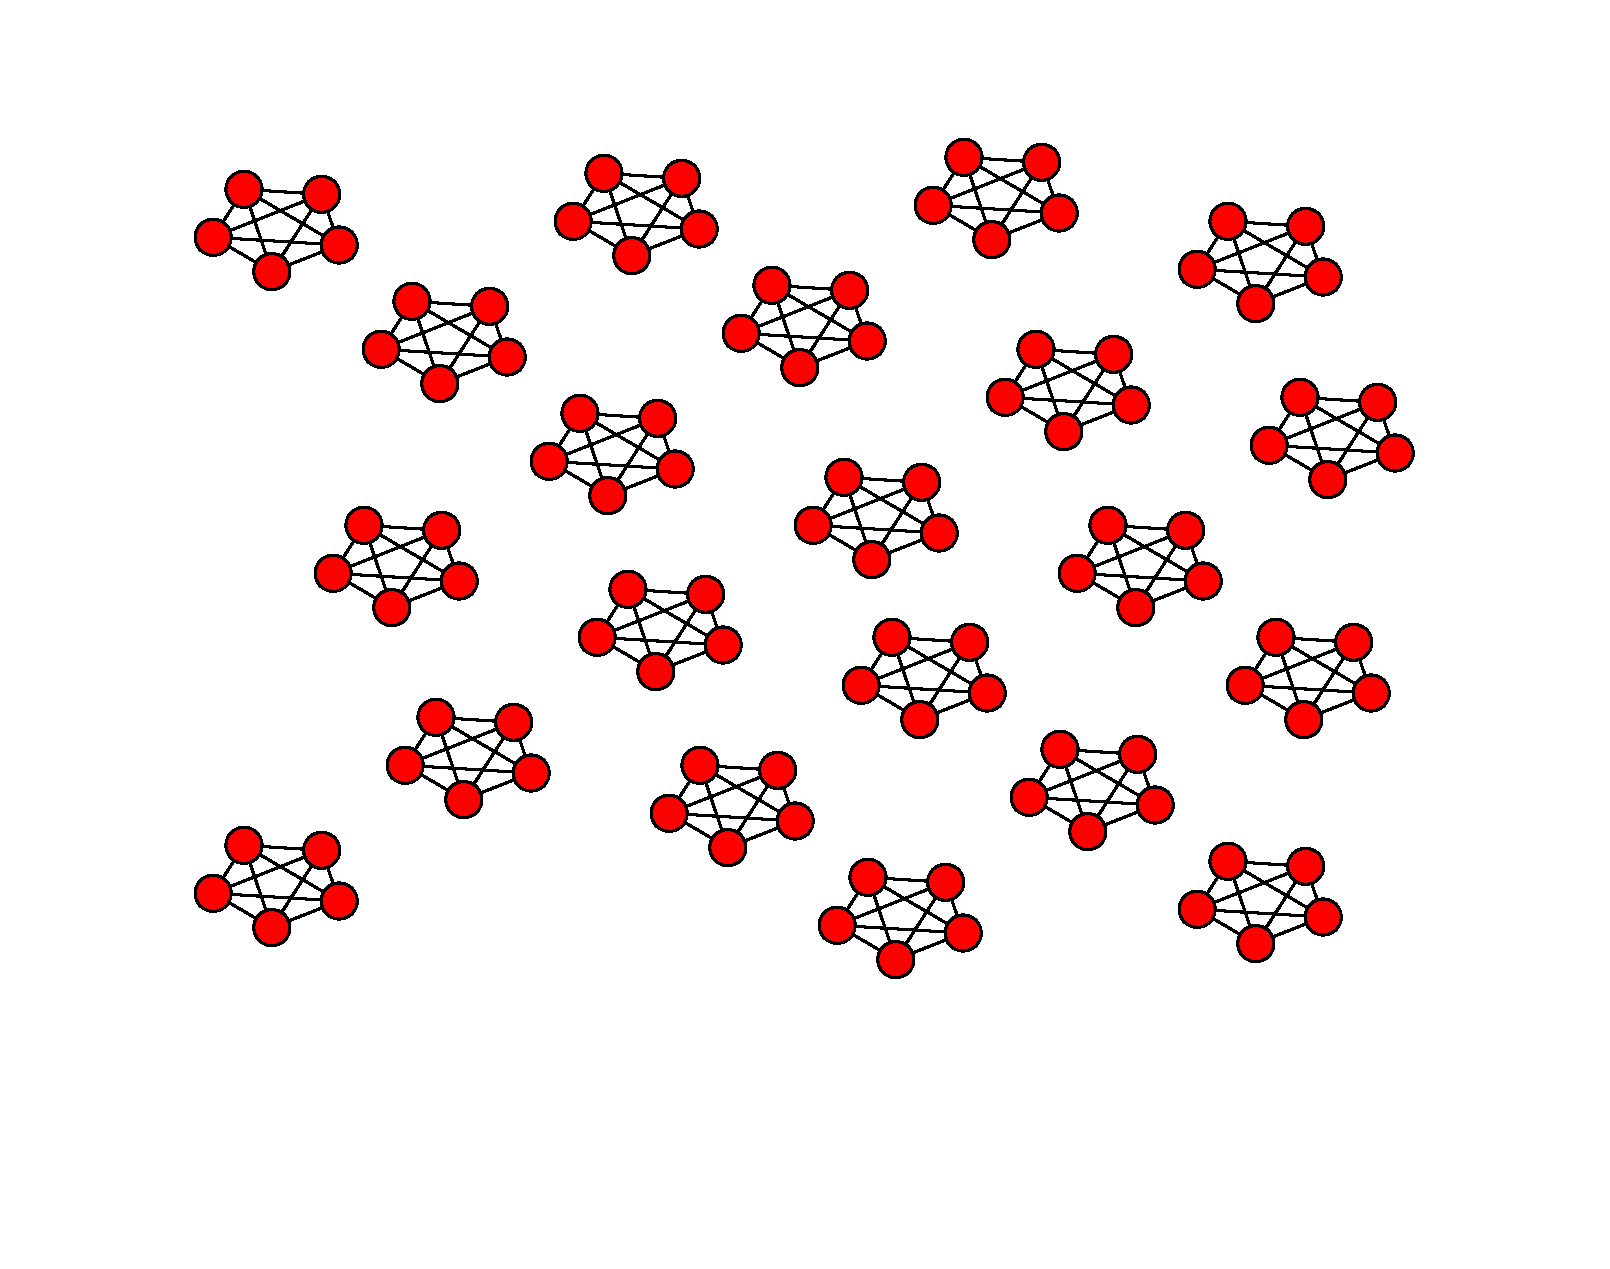
\includegraphics[width=\textwidth]{images/topology/fixed_patch_graph.pdf}
                \caption{The graphu}
        \end{subfigure}
        \begin{subfigure}[b]{0.4\textwidth}
        	\centering
                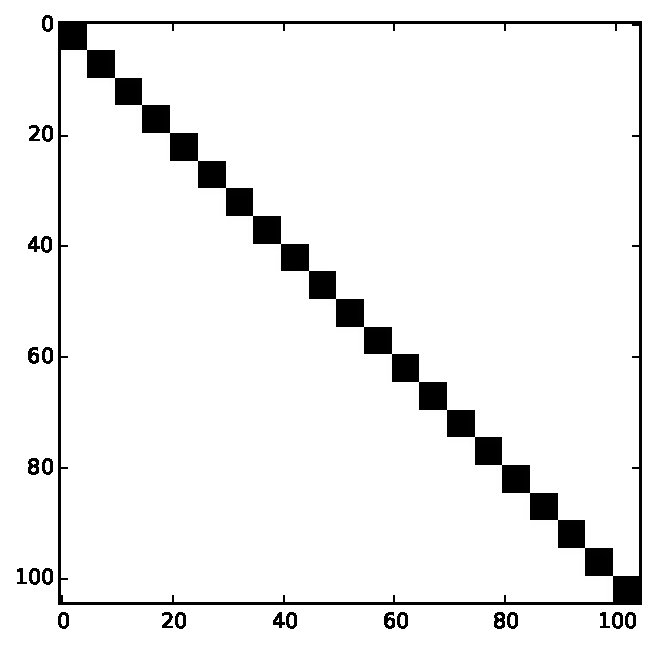
\includegraphics[width=\textwidth]{images/topology/fixed_patch_adjacency.pdf}
                \caption{The adjacency matrix}
                \label{subfig:fixed adjacency}
        \end{subfigure}
        \caption{Graph and the adjacency matrix of a set of 101 agents divided into 21 fixed one-dimensional communities}
        \label{fig:fixed adjacency graph}
\end{figure}

An example network generated by this division is shown in Figure \ref{fig:fixed adjacency graph}, were the isolation of communities from each other is clearly visible.
The same result can be seen by looking at the adjacency matrix in subfigure \ref{subfig:fixed adjacency}.

\section{Sliding window communities}
\label{sec:sliding communities}

To overcome the difficulty of having isolated communities we take different approach and create a community for each agent.
This is more representative of real world cases and also of the way minority games are defined.

Sliding window technique is used to create communities by creating a local neighbourhood for each agent.
Another possibility opens up here in deciding how many dimension we want to use to represent the set of agents.
We have used one-dimensional arrays and two-dimensional matrix to group agents into communities, and have not delved in higher dimensions as it does not bring any qualitative change, only modifies the graphical representation of agents.

\subsection{Sliding window on one-dimensional array}
\label{subsec:sliding}

Let's assume $N$ is the number of agents and $V$ is an odd integer representing the number of neighbours in each community.
For each agent $a_i$ a community $C_i$ is created from a sliding window of length $V$ centred on agent $a_i$.
an example of this simple procedure can be seen in figure \ref{fig:sliding window one-dimension}

\begin{figure}
\begin{center}
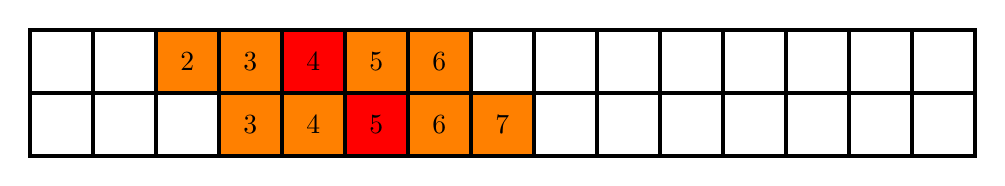
\begin{tikzpicture}[scale=0.8]
\draw [ultra thick] (0,0) rectangle (1,1);
\draw [ultra thick] (1,0) rectangle (2,1);
\draw [ultra thick] (2,0) rectangle (3,1);
\draw [fill=orange,ultra thick] (3,0) rectangle (4,1);
\draw [fill=orange,ultra thick] (4,0) rectangle (5,1);
\draw [fill=red,ultra thick] (5,0) rectangle (6,1);
\draw [fill=orange,ultra thick] (6,0) rectangle (7,1);
\draw [fill=orange,ultra thick] (7,0) rectangle (8,1);
\draw [ultra thick] (8,0) rectangle (9,1);
\draw [ultra thick] (9,0) rectangle (10,1);
\draw [ultra thick] (10,0) rectangle (11,1);
\draw [ultra thick] (11,0) rectangle (12,1);
\draw [ultra thick] (12,0) rectangle (13,1);
\draw [ultra thick] (13,0) rectangle (14,1);
\draw [ultra thick] (14,0) rectangle (15,1);

\draw [ultra thick] (0,1) rectangle (1,2);
\draw [ultra thick] (1,1) rectangle (2,2);
\draw [fill=orange,ultra thick] (2,1) rectangle (3,2);
\draw [fill=orange,ultra thick] (3,1) rectangle (4,2);
\draw [fill=red,ultra thick] (4,1) rectangle (5,2);
\draw [fill=orange,ultra thick] (5,1) rectangle (6,2);
\draw [fill=orange,ultra thick] (6,1) rectangle (7,2);
\draw [ultra thick] (7,1) rectangle (8,2);
\draw [ultra thick] (8,1) rectangle (9,2);
\draw [ultra thick] (9,1) rectangle (10,2);
\draw [ultra thick] (10,1) rectangle (11,2);
\draw [ultra thick] (11,1) rectangle (12,2);
\draw [ultra thick] (12,1) rectangle (13,2);
\draw [ultra thick] (13,1) rectangle (14,2);
\draw [ultra thick] (14,1) rectangle (15,2);

\node at (2.5,1.5) {2};
\node at (3.5,1.5) {3};
\node at (4.5,1.5) {4};
\node at (5.5,1.5) {5};
\node at (6.5,1.5) {6};
\node at (3.5,.5) {3};
\node at (4.5,.5) {4};
\node at (5.5,.5) {5};
\node at (6.5,.5) {6};
\node at (7.5,.5) {7};
\end{tikzpicture}
\caption{Example of communities created using sliding window on one-dimensional array for agents 4 and 5 where each community consists of 5 agents}
\label{fig:sliding window one-dimension}
\end{center}
\end{figure}

\begin{figure}[h]
        \centering
        \begin{subfigure}[b]{0.5\textwidth}
        	\centering
                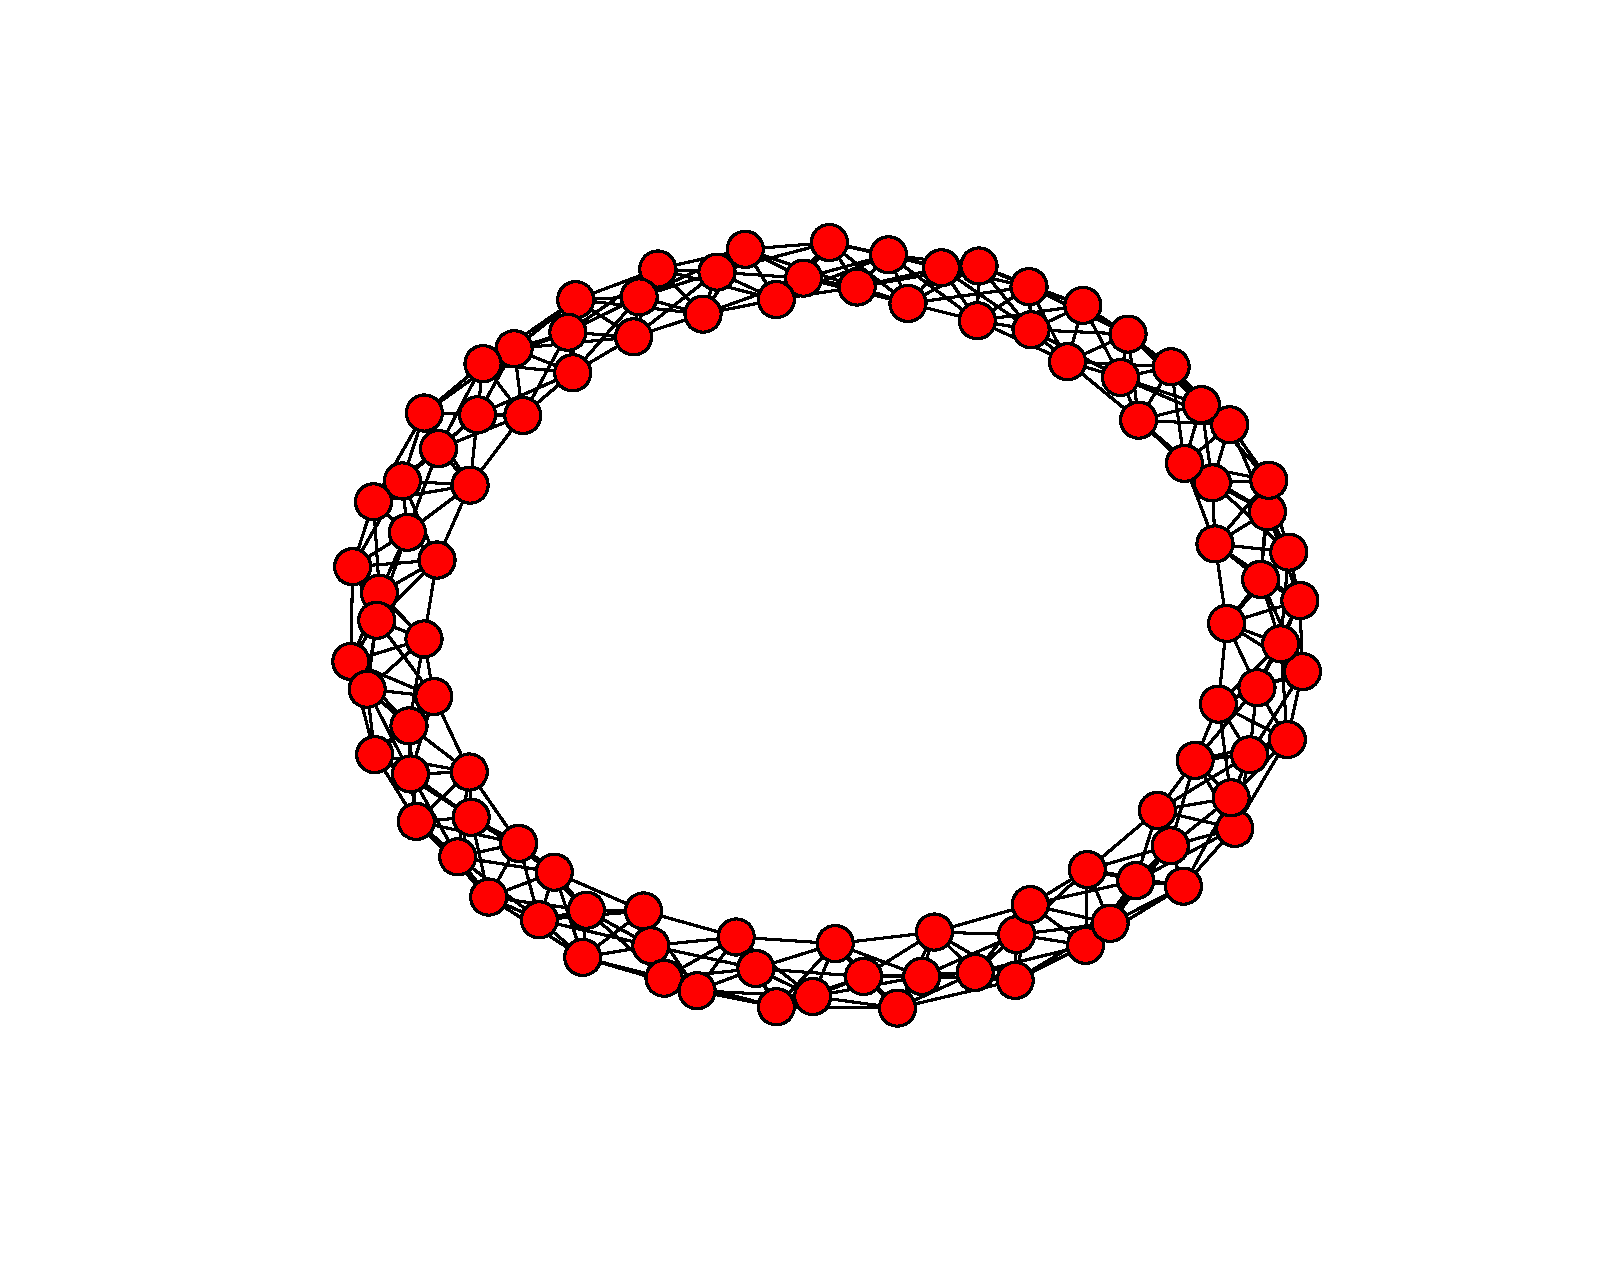
\includegraphics[width=\textwidth]{images/topology/sliding_window_graph.pdf}
                \caption{The graph}
        \end{subfigure}
        \begin{subfigure}[b]{0.4\textwidth}
        	\centering
                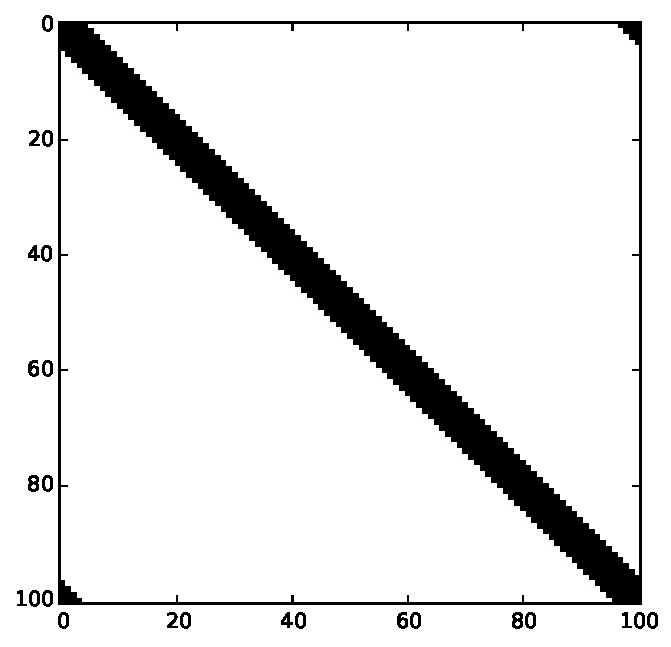
\includegraphics[width=\textwidth]{images/topology/sliding_window_adjacency.pdf}
                \caption{The adjacency matrix}
                \label{subfig:sliding adjacency}
        \end{subfigure}
        \caption{Graph and the adjacency matrix of a set of 101 agents divided into 101 sliding window one-dimensional communities}
        \label{fig:sliding adjacency graph}
\end{figure}

The network created in this way allows the information to flow between communities.
This kind of behaviour renders the efficient use of information more difficult when minority games are concerned, but it is more representative of human and human-made systems.
An example of a network can be seen in Figure \ref{fig:sliding adjacency graph} where the graph of a model with 101 agents, with each agent having a community of 5 neighbours, and the adjacency matrix are drawn.

\subsection{Sliding window on a matrix}

Different approach is to represent agents in two-dimensional array and construct neighbourhoods on the matrix generated.
This opens possibilities to use different rules for generating the vicinity, such as using the Manhattan distance to generate von Neumann vicinity as described in \ref{sec:von neumann}.
Another simple metric that can be used to generate neighbourhood is Chebyshev distance.
The Chebyshev distance, named after Pafnuty Chebyshev, also called chessboard distance, is defined as the greatest difference of distance along any coordinate dimension between two vectors.

\begin{displaymath}
D_{Chebyshev}(p,q) := max_i (|p_i-q_i|) 
\end{displaymath}

For each agent a community is generated that includes all agents with $D_{Chebyshev}$ less or equal than $R$, where $R$ is the radius of the neighbourhood.

\begin{figure}
        \centering
        \begin{subfigure}[b]{0.3\textwidth}
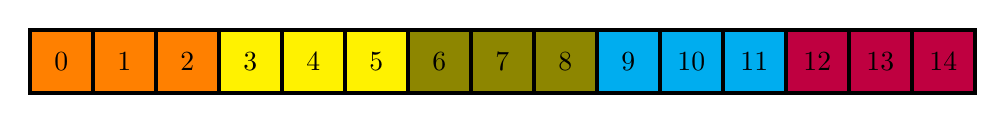
\begin{tikzpicture}[scale=0.8]
\draw [fill=orange,ultra thick] (0,0) rectangle (1,1);
\draw [fill=orange,ultra thick] (1,0) rectangle (2,1);
\draw [fill=orange,ultra thick] (2,0) rectangle (3,1);
\draw [fill=yellow,ultra thick] (3,0) rectangle (4,1);
\draw [fill=yellow,ultra thick] (4,0) rectangle (5,1);
\draw [fill=yellow,ultra thick] (5,0) rectangle (6,1);
\draw [fill=olive,ultra thick] (6,0) rectangle (7,1);
\draw [fill=olive,ultra thick] (7,0) rectangle (8,1);
\draw [fill=olive,ultra thick] (8,0) rectangle (9,1);
\draw [fill=cyan,ultra thick] (9,0) rectangle (10,1);
\draw [fill=cyan,ultra thick] (10,0) rectangle (11,1);
\draw [fill=cyan,ultra thick] (11,0) rectangle (12,1);
\draw [fill=purple,ultra thick] (12,0) rectangle (13,1);
\draw [fill=purple,ultra thick] (13,0) rectangle (14,1);
\draw [fill=purple,ultra thick] (14,0) rectangle (15,1);

\node at (0.5,.5) {0};
\node at (1.5,.5) {1};
\node at (2.5,.5) {2};
\node at (3.5,.5) {3};
\node at (4.5,.5) {4};
\node at (5.5,.5) {5};
\node at (6.5,.5) {6};
\node at (7.5,.5) {7};
\node at (8.5,.5) {8};
\node at (9.5,.5) {9};
\node at (10.5,.5) {10};
\node at (11.5,.5) {11};
\node at (12.5,.5) {12};
\node at (13.5,.5) {13};
\node at (14.5,.5) {14};
\end{tikzpicture}
                \caption{A gull}
                \label{fig:gull}
        \end{subfigure}%
        ~ %add desired spacing between images, e. g. ~, \quad, \qquad, \hfill etc.
          %(or a blank line to force the subfigure onto a new line)
        \begin{subfigure}[b]{0.3\textwidth}
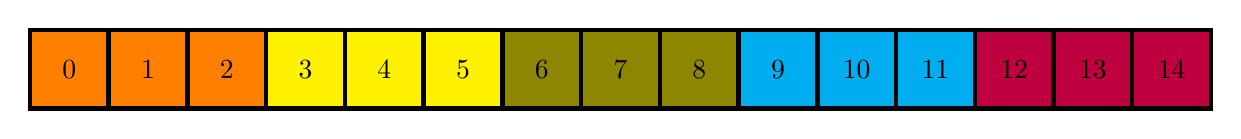
\begin{tikzpicture}
\draw [fill=orange,ultra thick] (0,0) rectangle (1,1);
\draw [fill=orange,ultra thick] (1,0) rectangle (2,1);
\draw [fill=orange,ultra thick] (2,0) rectangle (3,1);
\draw [fill=yellow,ultra thick] (3,0) rectangle (4,1);
\draw [fill=yellow,ultra thick] (4,0) rectangle (5,1);
\draw [fill=yellow,ultra thick] (5,0) rectangle (6,1);
\draw [fill=olive,ultra thick] (6,0) rectangle (7,1);
\draw [fill=olive,ultra thick] (7,0) rectangle (8,1);
\draw [fill=olive,ultra thick] (8,0) rectangle (9,1);
\draw [fill=cyan,ultra thick] (9,0) rectangle (10,1);
\draw [fill=cyan,ultra thick] (10,0) rectangle (11,1);
\draw [fill=cyan,ultra thick] (11,0) rectangle (12,1);
\draw [fill=purple,ultra thick] (12,0) rectangle (13,1);
\draw [fill=purple,ultra thick] (13,0) rectangle (14,1);
\draw [fill=purple,ultra thick] (14,0) rectangle (15,1);

\node at (0.5,.5) {0};
\node at (1.5,.5) {1};
\node at (2.5,.5) {2};
\node at (3.5,.5) {3};
\node at (4.5,.5) {4};
\node at (5.5,.5) {5};
\node at (6.5,.5) {6};
\node at (7.5,.5) {7};
\node at (8.5,.5) {8};
\node at (9.5,.5) {9};
\node at (10.5,.5) {10};
\node at (11.5,.5) {11};
\node at (12.5,.5) {12};
\node at (13.5,.5) {13};
\node at (14.5,.5) {14};
\end{tikzpicture}
                \caption{A tiger}
                \label{fig:tiger}
        \end{subfigure}

        \caption{Pictures of animals}\label{fig:animals}
\end{figure}

\section{Von Neumann Vicinity}
\label{sec:von neumann}

Along with the chessboard metric, Manhattan distance is another option when constructing vicinities.
Called also taxicab distance, this metric is defined as the sum of the lengths of the projections of the line segment between the points onto the coordinate axes.
\begin{displaymath}
d_1(p,q) = ||p-q||_1 = \sum_{i=1}^n |p_i - q_i|
\end{displaymath}

The vicinity is constructed by using a sliding window mechanism on a two-dimensional matrix of agents.
For each agent $p$ is composed by a set of agents $q$ such that $d_1(p,q)$ is less than or equal to $R$, where $R$ is the radius of the von Neumann neighbourhood.
Such vicinities, with $R$ equal to 1 and 2, are shown in \ref{fig:vonNeumann}.

\begin{figure}
        \centering
        \begin{subfigure}[b]{0.4\textwidth}
\centering

\begin{tikzpicture}[scale=0.6]
\foreach \y in {0,...,4}
	\foreach \x in {0,...,4} {
		\ifthenelse{\x=2 \AND \y>0 \AND \y<4}{\def\mycol{orange}}{\def\mycol{white}}
		\ifthenelse{\x=2 \AND \y=2}{\def\mycol{red}}{}
		\ifthenelse{\x=1 \AND \y=2}{\def\mycol{orange}}{}
		\ifthenelse{\x=3 \AND \y=2}{\def\mycol{orange}}{}
		\draw [fill=\mycol](\x, \y) rectangle (\x+1,\y+1);
	}
\end{tikzpicture}
                \caption{Radius 1}
                \label{fig:gull}
        \end{subfigure}
        \begin{subfigure}[b]{0.5\textwidth}
\centering

\begin{tikzpicture}[scale=0.6]
\foreach \y in {0,...,6}
	\foreach \x in {0,...,6} {
		\ifthenelse{\x>1 \AND \x<5 \AND \y>1 \AND \y<5}{\def\mycol{orange}}{\def\mycol{white}}
		\ifthenelse{\x=3 \AND \y=3}{\def\mycol{red}}{}
		\ifthenelse{\x=1 \AND \y=3}{\def\mycol{orange}}{}
		\ifthenelse{\x=3 \AND \y=1}{\def\mycol{orange}}{}
		\ifthenelse{\x=3 \AND \y=5}{\def\mycol{orange}}{}
		\ifthenelse{\x=5 \AND \y=3}{\def\mycol{orange}}{}
		\draw [fill=\mycol](\x, \y) rectangle (\x+1,\y+1);
	}
\end{tikzpicture}
                \caption{Radius 2}
                \label{fig:tiger}
        \end{subfigure}

        \caption{von Neumann vicinity with radius 1 and 2}\label{fig:vonNeumann}
\end{figure}

\begin{figure}[h]
        \centering
        \begin{subfigure}[b]{0.5\textwidth}
        	\centering
                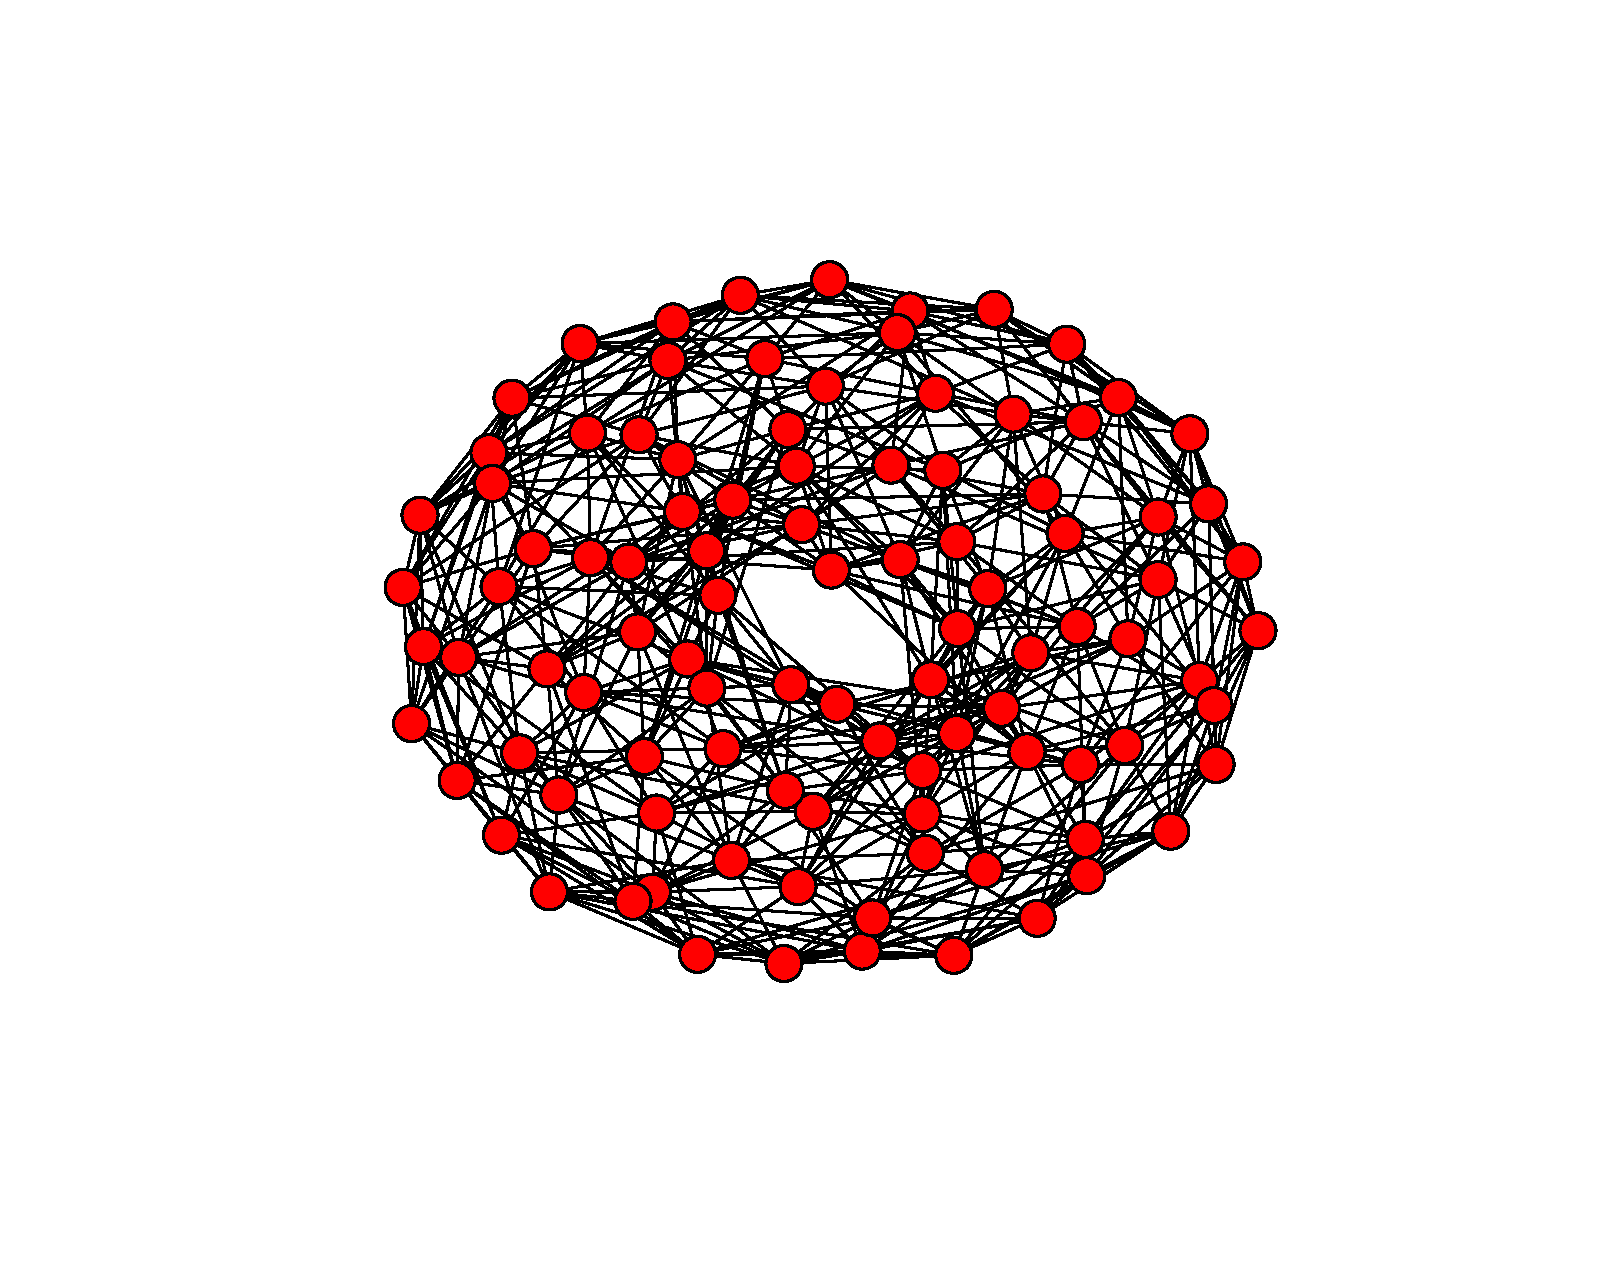
\includegraphics[width=\textwidth]{images/topology/von_neumann_graph.pdf}
                \caption{The graph}
        \end{subfigure}
        \begin{subfigure}[b]{0.4\textwidth}
        	\centering
                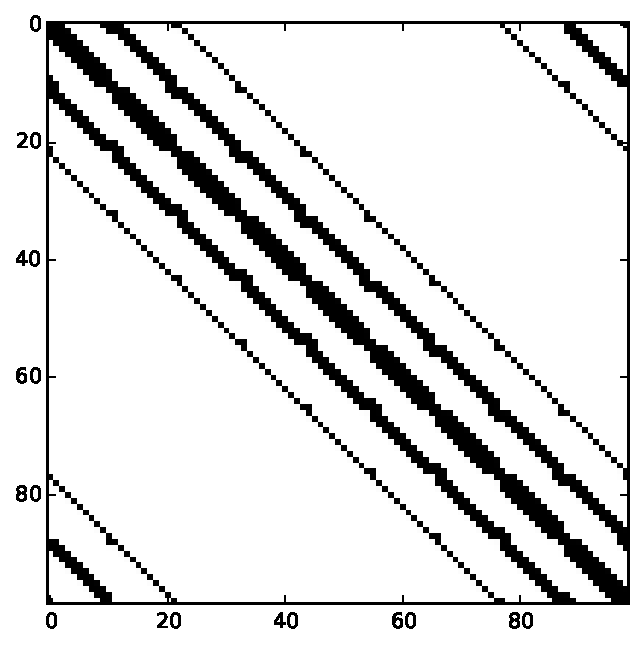
\includegraphics[width=\textwidth]{images/topology/von_neumann_adjacency.pdf}
                \caption{The adjacency matrix}
                \label{subfig:vonNeumann adjacency}
        \end{subfigure}
        \caption{Graph and the adjacency matrix of a set of 101 agents divided into 101 von Neumann two-dimensional communities with $R=2$}
        \label{fig:vonNeumann adjacency graph}
\end{figure}

The main distinction between using a one-dimensional array or two-dimensional matrix to represent the set of agents is that more possible metrics for constructing the vicinity are available as the dimensions get higher.
The downside of higher dimension vicinities is that usually the number of agents included in the neighbourhood is fixed.
For example, when constructing von Neumann vicinities the number of agents inside the community is $5$ if $R=1$ is used, $13$ if $R=2$ is used, $41$ for $R=3$ and so on.
This sort of progression can prove to be inadequate when we want to study the dynamics of a system based on the number of agents in the communities.
A more contained approach that enables us to study the model while increasing the number of neighbours in a linear fashion is more favourable.

The graph defined by agents as nodes and where edges represent the membership of two agents to the same community can be seen in Figure \ref{fig:vonNeumann adjacency graph}, while the adjacency matrix is shown in subfigure \ref{subfig:vonNeumann adjacency}.
The graph exhibits similar properties to the graph defined by one-dimensional sliding window vicinities, with the difference that the communities consist of more agents, as $R=2$ is used, ie. neighbourhood consists of $13$ agents.
The adjacency matrix seems to exhibit different characteristics, but the difference is mainly due to the fact that the vicinity is constructed on a two-dimensional matrix instead of a one-dimensional array.
The qualitative properties do not show significant change between different dimensional approaches.

\section{Scale free network vicinities}
\label{sec:scale free}

Scale free networks are characterized by a degree distribution, ie. the connectivity of nodes, as a power law. This means that the probability of an agent having $k$ neighbours follows
\begin{displaymath}
P(k) \sim k^{-\gamma}
\end{displaymath}

The scale free properties are observed in many ecosystems that are the subject of this thesis, as social networks, financial markets and computer networks.
The assumption used to generate and explain these kinds of network is called preferential attachment.
This mechanism explains how when new nodes are added to the network they are more likely to connect to a node with high degree, rather than to a unknown node.
Example of a computer network is the network of links between websites, where when new website is created it is more probable it will contain links to well known websites such as Wikipedia, rather than to some obscure nodes of the network. 
In human networks we can think of financial agents and agencies as nodes and the flow of information between them as nodes. 
As new agents enter the market they will probably be more interested in connecting to, ie. obtaining information from, a well known agency than from some obscure sources.

To construct an artificial scale-free network a Barabasi-Albert algorithm \cite{albert2002statistical} is used. 
The network is initiated with $n_0$ connected nodes and new nodes are added one at a time.
When generating the network, aside from the number of total nodes, a number $e$ of edges per node is given.
Each time a node is added it is connected to $e$ nodes with probability of being connected to node $i$ equal to

\begin{displaymath}
p_i = \frac{k_i}{\sum_j k_j}
\end{displaymath}

where $k_i$ is the degree of node $i$.

\begin{figure}[h]
        \centering
        \begin{subfigure}[b]{0.5\textwidth}
        	\centering
                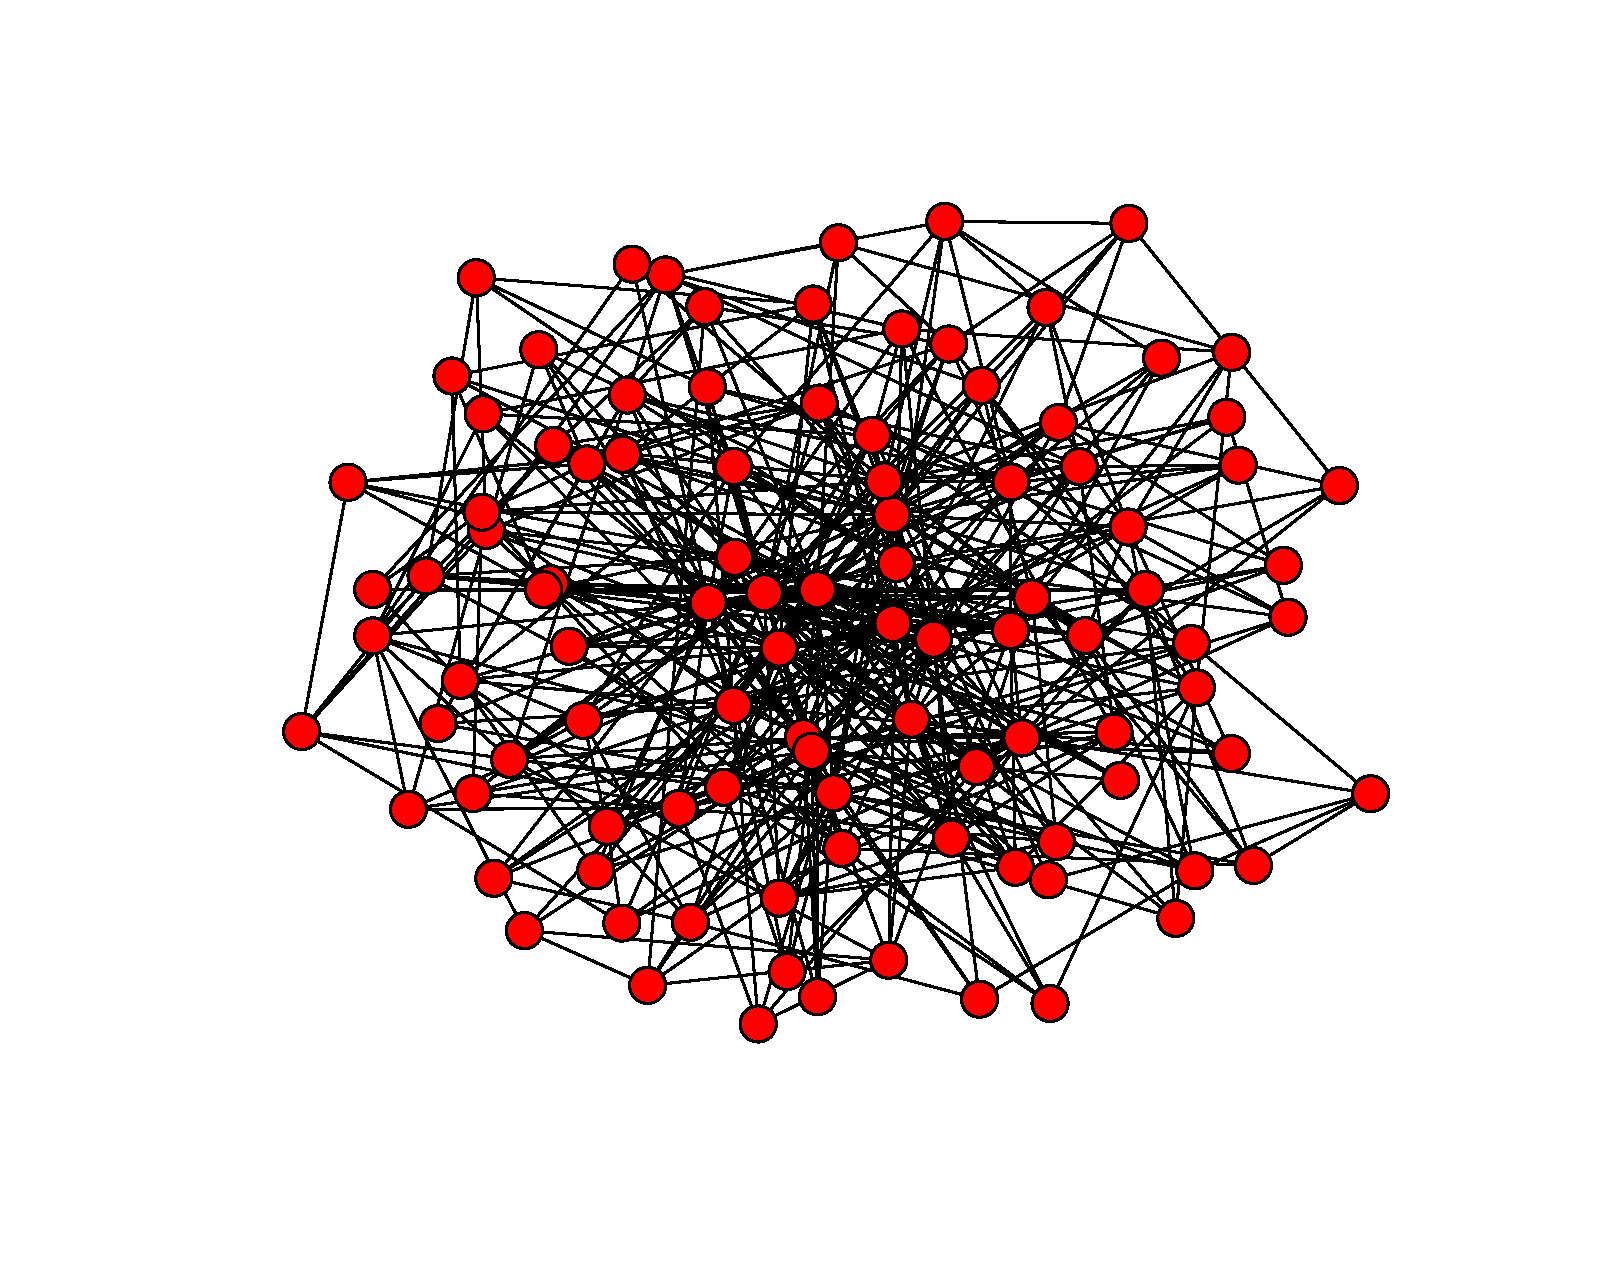
\includegraphics[width=\textwidth]{images/topology/scale_free_barabasi_graph.pdf}
                \caption{The graph}
        \end{subfigure}
        \begin{subfigure}[b]{0.4\textwidth}
        	\centering
                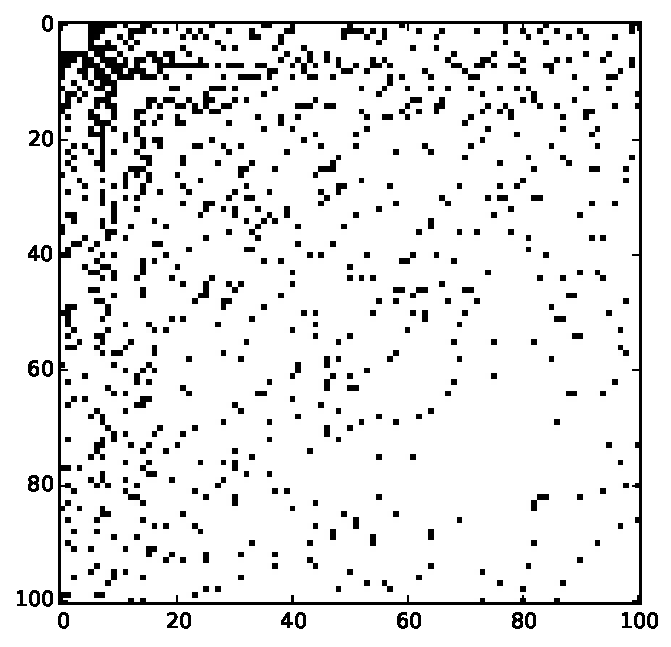
\includegraphics[width=\textwidth]{images/topology/scale_free_barabasi_adjacency.pdf}
                \caption{The adjacency matrix}
                \label{subfig:scale free adjacency}
        \end{subfigure}
        \caption{Scale free graph and the adjacency matrix of a set of 101 agents}
        \label{fig:scale free adjacency graph}
\end{figure}

We have opted to use this network structure because it closely models some of the systems that we are trying to optimize.
An example graph constructed with Barabasi-Albert algorithm can be seen in Figure \ref{fig:scale free adjacency graph}.
Event though the number of nodes and edges makes it more difficult to see the nature of the graph, it can be noted that central nodes, called \textit{hubs}, are the ones more connected than the peripheral ones.
This property can be more easily seen examining the adjacency matrix of the graph, in subfigure \ref{subfig:scale free adjacency}, where it is obvious that the nodes that are added initially are the ones well connected and become \textit{hubs} as the graph is populated.

\section{Small world network vicinities}
\label{sec:small world}

Small world networks are a type of graphs where most of the nodes are not the neighbours of each other but are easily reachable with a limited number of hops.
They have been introduced by Duncan Watts and Steven Strogatz in their joint work \cite{watts1998collective} and the two main characteristics of such a network are short average path length between nodes, and high clustering effect.
The average number of hops required to reach node $j$ starting from node $i$ grows as a logarithm of the total number of agents, ie. $L \propto log(N)$ and hence the first property.
The second property is obtained through the network generation proposed by Watts and Strogatz that differs from previously presented random generation algorithms.

Small world networks have been observed in social networks as well as other ecosystems, human-made and natural.
In the social network context the small world properties of short average node-to-node distance and high clustering are a result of strangers being linked through mutual acquaintances, and communities clustering in same space and time.
The probability of two persons being linked directly is significantly higher if they inhabit the same community (or city, country, etc.) as well as if they are close in time, ie. similar age, hence explained the clustering effect.

Watts and Strogatz algorithm to generate small world network takes in input the number of nodes $N$, average degree of a node $K$ and the special parameter $\beta$ such that $0\leq \beta \leq 1$ and $N\gg K\gg ln(N) \gg 1$.
The graph is constructed by first creating a regular lattice ring, a set of nodes $N$ each connected to the $K/2$ neighbours before and after if a set of nodes is represented as an array.
This mechanism is the same as the one describes as a one-dimensional sliding window in Section \ref{sec:sliding communities}.
After the first step for every node $n_i$ every edge $(n_i,n_j)$ is taken and rewired with probability $\beta$. The rewiring is done by replacing $(n_i,n_j)$ with $(n_i,n_k)$ where $k$ is chosen randomly until a condition that $k\neq k'$ if $(n_i,n_{k'})$ exists.

Since there is still debate as to whether different social and computer networks are better modelled with scale-free or small world graphs, both have been used to study how their structure influences the community minority games.
With small world we can expect that the information is used rather efficiently as the agents are clustered into local communities, and that some flow of information is permitted through the rewired nodes between different communities.

An example of a small world graph can be seen in Figure \ref{fig:small world adjacency graph}.
Better understanding of this network is obtained if we look at the adjacency matrix in subfigure \ref{subfig:small world adjacency}, where we can see the resemblance with the sliding window techniques, and the randomness introduced by the parameter $\beta$.
For different values of $\beta$, the similarity with sliding window vicinities changes, as can be seen in Figure \ref{fig:small world 25} where for a low probability of rewiring the resemblance is greater that in the case shown in subfigure \ref{subfig:small world adjacency}  where $\beta = 0.75$.

\begin{figure}[h]
        \centering
        \begin{subfigure}[b]{0.5\textwidth}
        	\centering
                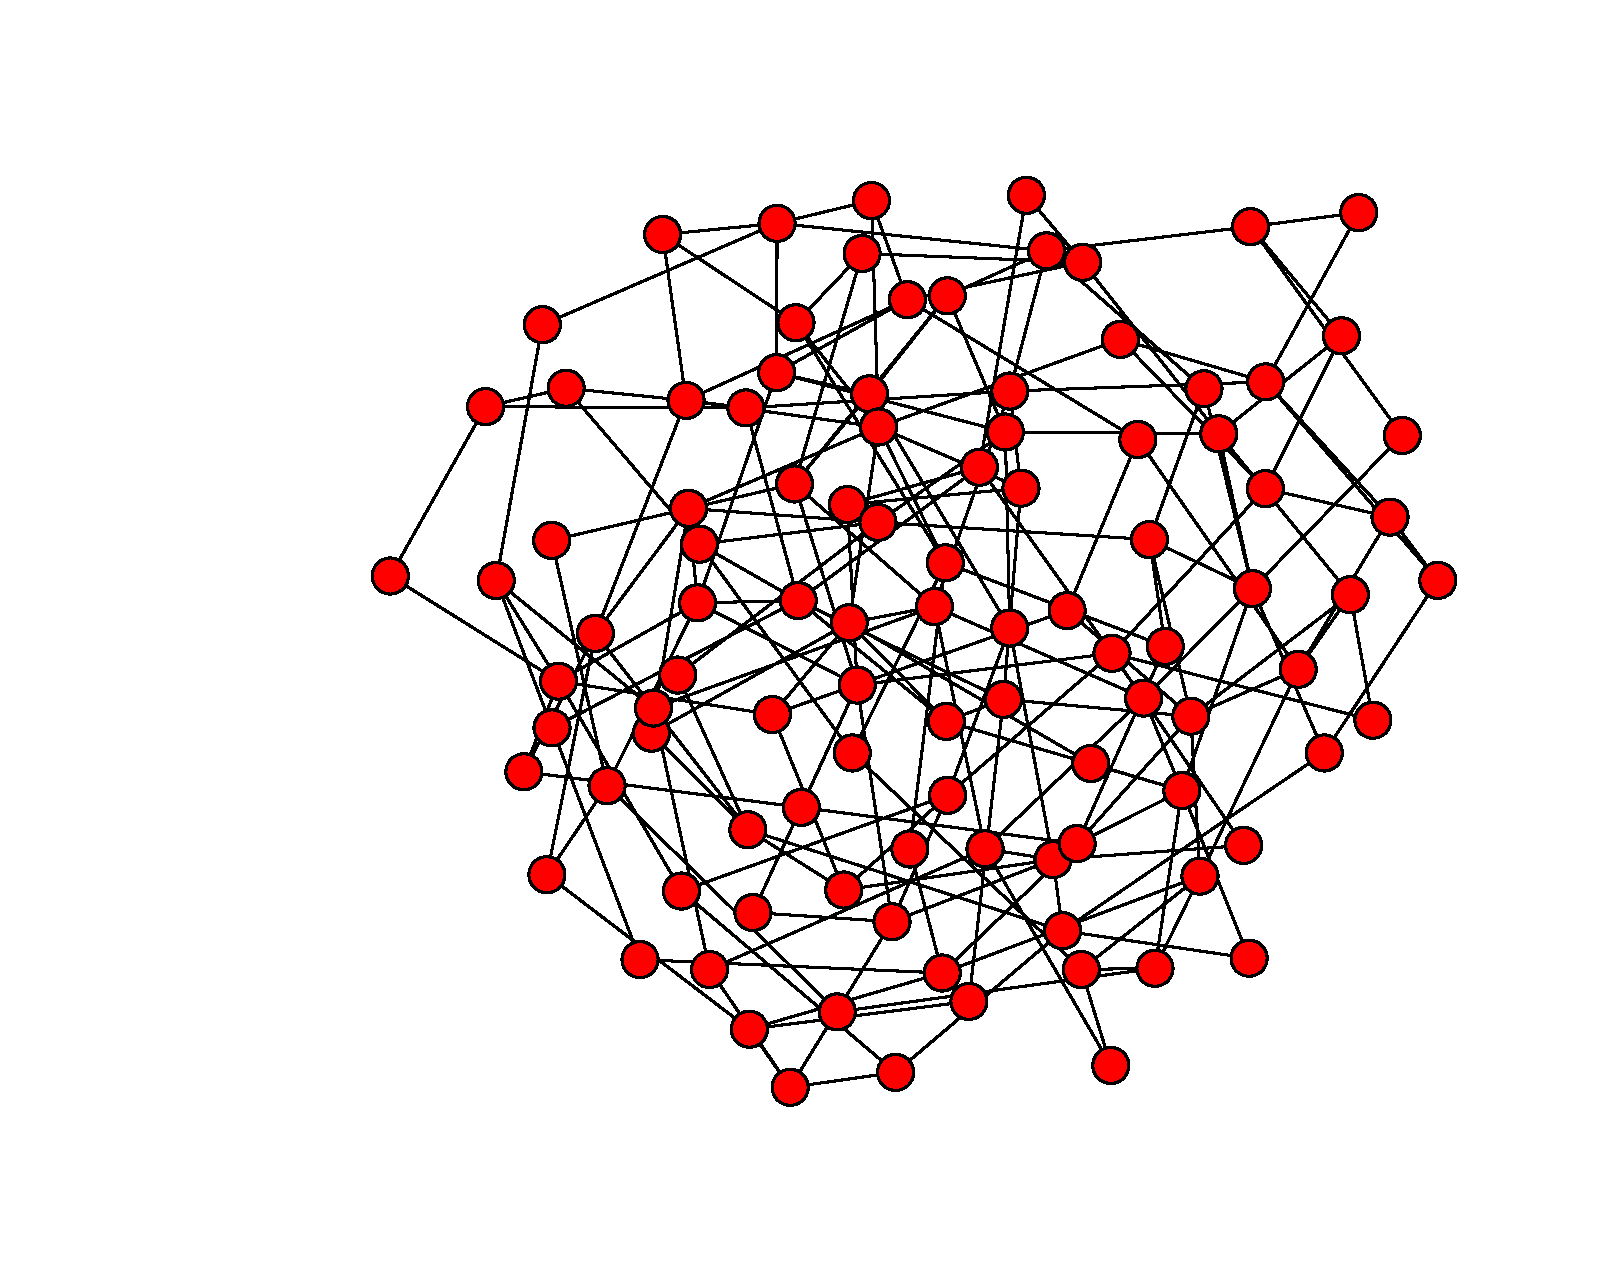
\includegraphics[width=\textwidth]{images/topology/small_world_watts_graph.pdf}
                \caption{The graph}
        \end{subfigure}
        \begin{subfigure}[b]{0.4\textwidth}
        	\centering
                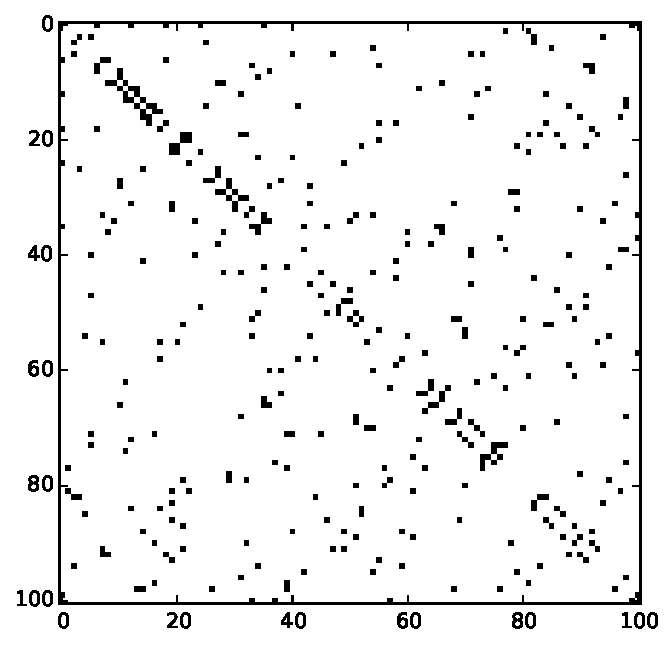
\includegraphics[width=\textwidth]{images/topology/small_world_watts_adjacency_75.pdf}
                \caption{The adjacency matrix}
                \label{subfig:small world adjacency}
        \end{subfigure}
        \caption{Small world graph and the adjacency matrix with $N=101$, $K=5$ and $\beta =0.75$}
        \label{fig:small world adjacency graph}
\end{figure}

\begin{figure}[h]
\centering
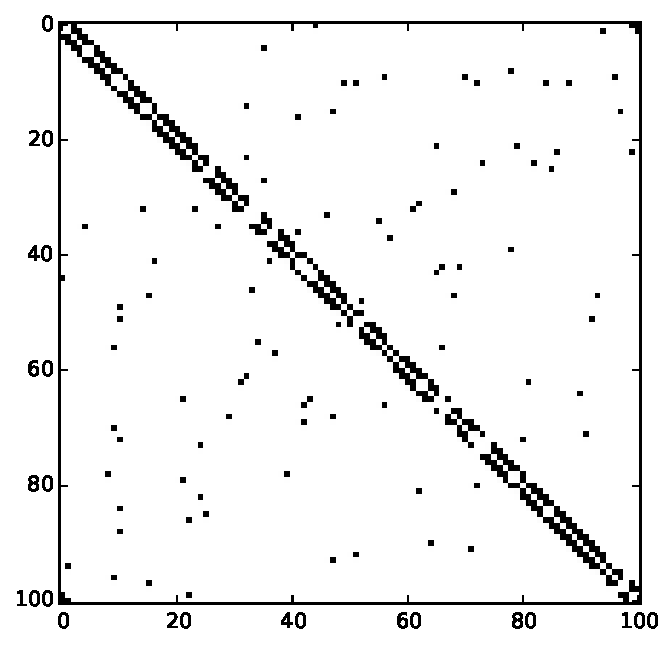
\includegraphics[scale=0.7]{images/topology/small_world_watts_adjacency_25.pdf}
\caption{Small world graph adjacency matrix with $N=101$, $K=5$ and $\beta = 0.25$}
\label{fig:small world 25}
\end{figure}

\section{Hierarchical vicinity structure}
\label{sec:hierarchical vicinity}

More complex small world and scale free graphs allow us to model more realistically human and computer networks, but they still have certain fallacies.
Scale free networks simulate the popularity effect through its peripheral attachment mechanism, making certain nodes more probable to have higher degree with respect to others.
However scale free network do not enable us to simulate high clustering around the whole network, clustering is generated only at the \textit{central} nodes, the ones with high degree.
On the other hand, small world graphs have high clustering property, intrinsic in it's algorithm definition, but the degree of each node is the same.

We find both approaches lacklustre, for within human networks as well as human-made we can observe the difference of link quantity between different nodes.
The peripheral attachment property seems present in most systems studied for the purpose of this thesis.
Likewise the clustering is also a real phenomenon, that can be observed easily in systems studied, for example the different branches of financial markets form loosely connected communities, divided whether by the object of their trading or by the place of their operation.

In an attempt to model competitive systems more closely we have decided to merge two different characteristics from small world and scale free graphs into a hybrid networks, that we call hierarchical network.
Single communities are formed by using the Barabasi-Albert algorithm in order to obtain the peripheral attachment property.
After $C$ communities have been generated they are united in a larger community and a second step of the Watts-Strogatz algorithm is executed to create a short average length between different communities.
If a high enough degree parameter is given to the Barabasi-Albert algorithm we can obtain locally high clustering, while maintaining the short average length between nodes with Watts-Strogatz application to the entire network.

\begin{figure}[h]
\centering
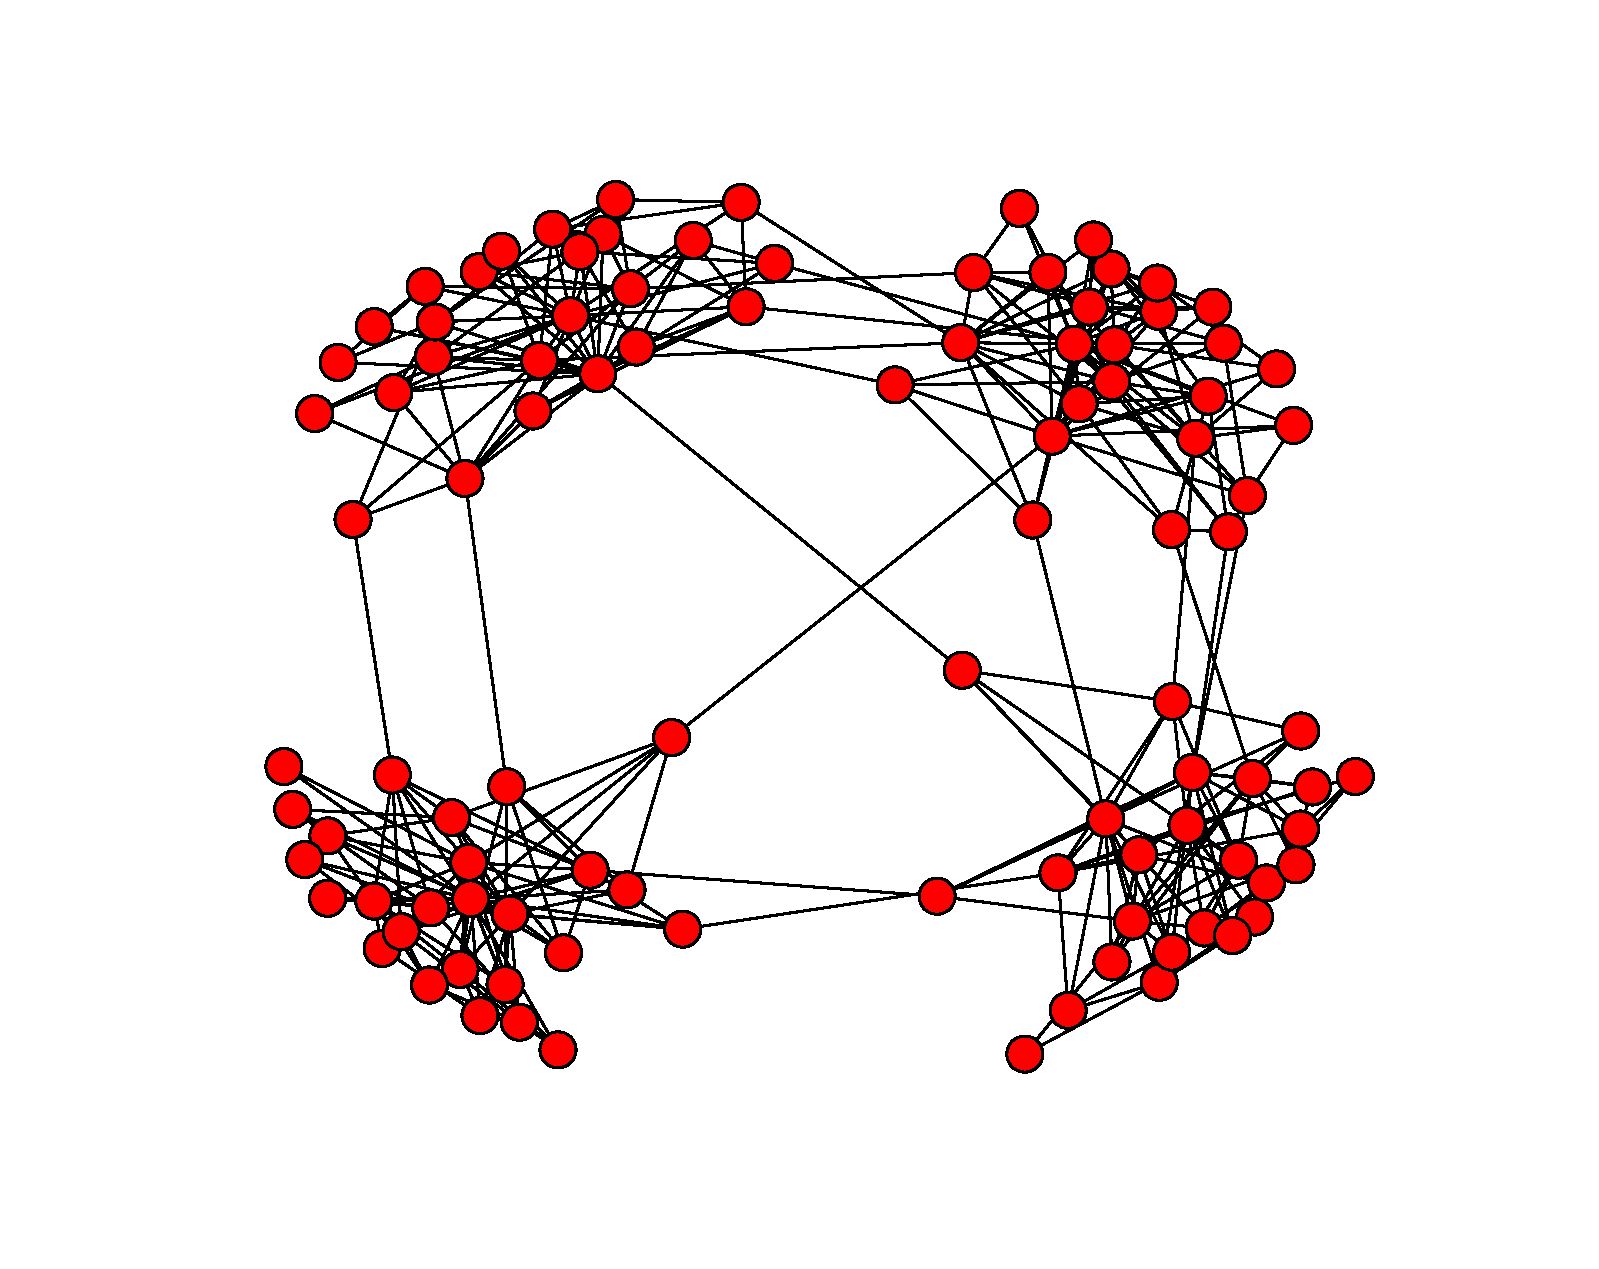
\includegraphics[scale=0.4]{images/topology/hierarchical_graph_4_dot05.pdf}
\caption{Hierarchical graph with $N=101$, $C=4$, $K=4$ and $\beta = 0.05$}
\label{fig:hierarchical graph 4}
\end{figure}

An example of a hierarchical graph can be seen in Figure \ref{fig:hierarchical graph 4} where $101$ initial agents are first divided into $4$ communities and then each edge is rewired with $\beta=0.05$ probability. 
The 4 communities are clearly visible and each community is loosely linked to each other maintaining low the short average path.

Same observation can be made by looking at the adjacency matrix of different hierarchical graphs.
Examples for hierarchical graphs with $C$ in $\{2,3,4\}$ for $\beta=0.1$ are visible in Figure  \ref{fig:hierarchical adjacency graph 0.1}, while for the same number of communities but with higher rewiring parameter $\beta=0.25$ can be seen in Figure \ref{fig:hierarchical adjacency graph 0.25}.

\begin{figure}[h]
        \centering
        \begin{subfigure}[b]{0.3\textwidth}
        	\centering
                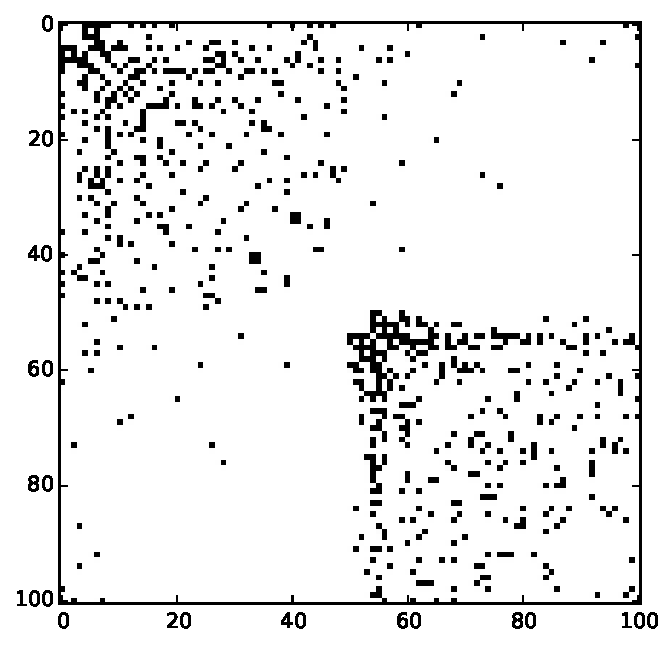
\includegraphics[width=\textwidth]{images/topology/hierarchical_adjacency_2_dot1.pdf}
                \caption{$C=2$}
        \end{subfigure}
        \begin{subfigure}[b]{0.3\textwidth}
        	\centering
                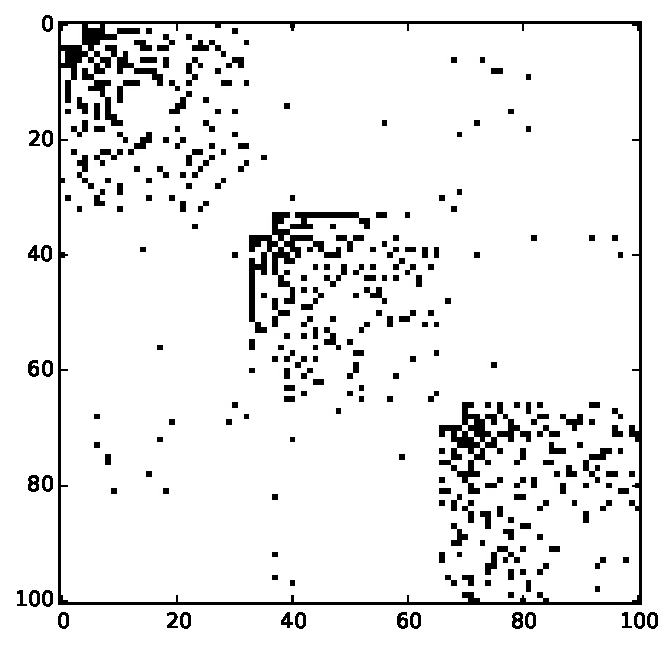
\includegraphics[width=\textwidth]{images/topology/hierarchical_adjacency_3_dot1.pdf}
                \caption{$C=3$}
        \end{subfigure}
        \begin{subfigure}[b]{0.3\textwidth}
        	\centering
                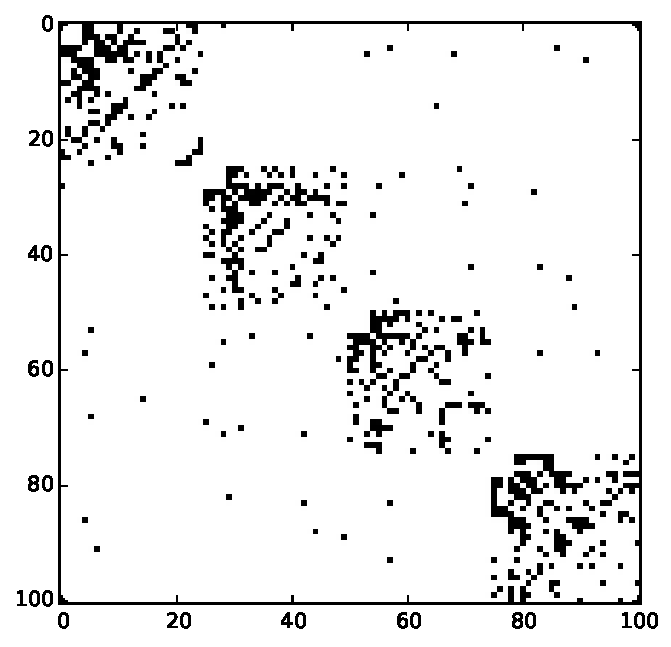
\includegraphics[width=\textwidth]{images/topology/hierarchical_adjacency_4_dot1.pdf}
                \caption{$C=4$}
        \end{subfigure}
        \caption{Hierarchical graph adjacency matrices with $N=101$, $K=5$ and $\beta =0.1$}
        \label{fig:hierarchical adjacency graph 0.1}
\end{figure}


\begin{figure}[h]
        \centering
        \begin{subfigure}[b]{0.3\textwidth}
        	\centering
                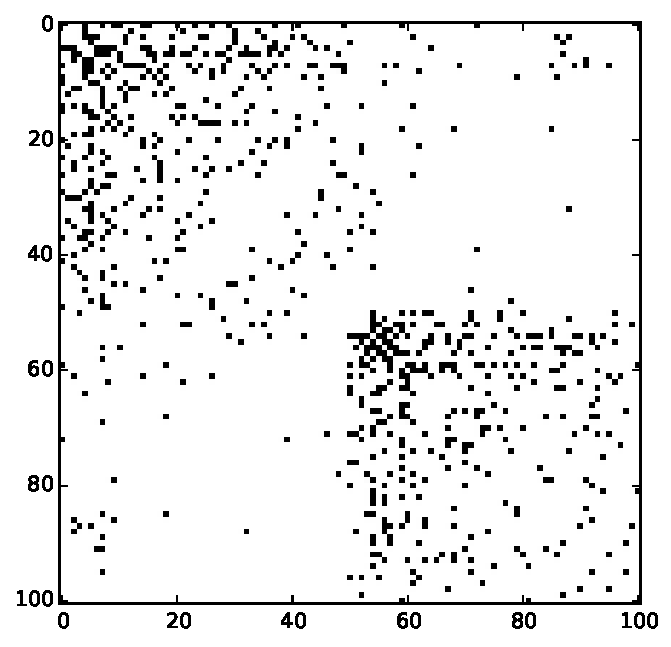
\includegraphics[width=\textwidth]{images/topology/hierarchical_adjacency_2_dot25.pdf}
                \caption{$C=2$}
        \end{subfigure}
        \begin{subfigure}[b]{0.3\textwidth}
        	\centering
                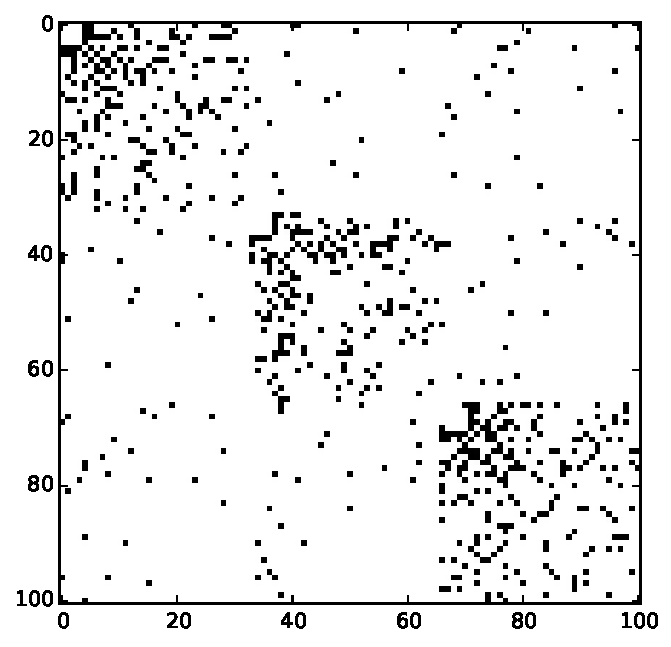
\includegraphics[width=\textwidth]{images/topology/hierarchical_adjacency_3_dot25.pdf}
                \caption{$C=3$}
        \end{subfigure}
        \begin{subfigure}[b]{0.3\textwidth}
        	\centering
                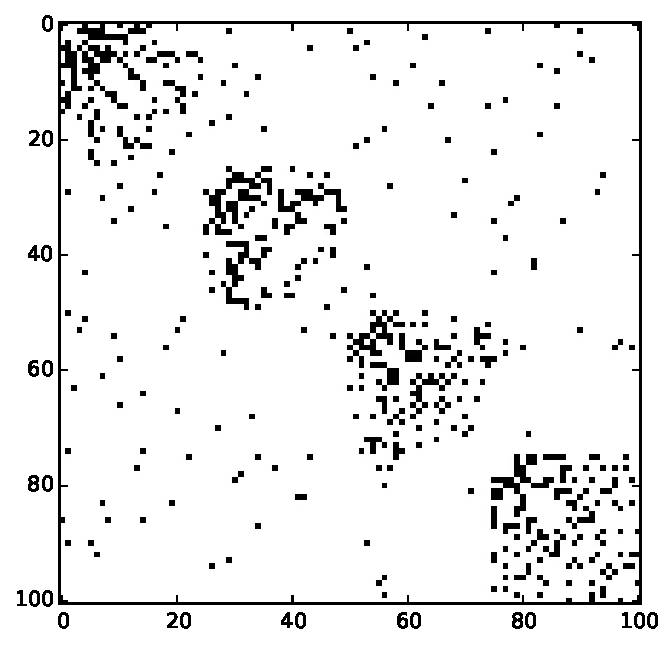
\includegraphics[width=\textwidth]{images/topology/hierarchical_adjacency_4_dot25.pdf}
                \caption{$C=4$}
        \end{subfigure}
        \caption{Hierarchical graph adjacency matrices with $N=101$, $K=5$ and $\beta =0.25$}
        \label{fig:hierarchical adjacency graph 0.25}
\end{figure}

We do not expect better or worse performance by using this structure for the vicinity in minority games, but the fact they are closely representative of real world network structures, we believe they need to be studied and analysed in order to find the best conditions under which these competitive systems perform.